\chapter{State-of-the-Art}\label{chap:sota}

\section{Animation of Single Characters}
\subsection{Sketch-Based Animation}
Guay et. al were the authors who originally proposed the line of action as a posing tool. In ``The Line of Action: an Intuitive Interface for Expressive Character Posing'' (\citep{guay2013line}), there were several contributions: adapting the line of action (LOA) in the form of a new notation to posing 3D characters, solving the LOA problem as an optimization problem, and validating this technique by having users recreate poses from images.

Their system, in which a user can draw a line in the shape they want a kinematic chain to take, works extremely well for a single humanoid character, and even multiple humanoid characters which are strictly separate from each other. 

\begin{figure}[!h]
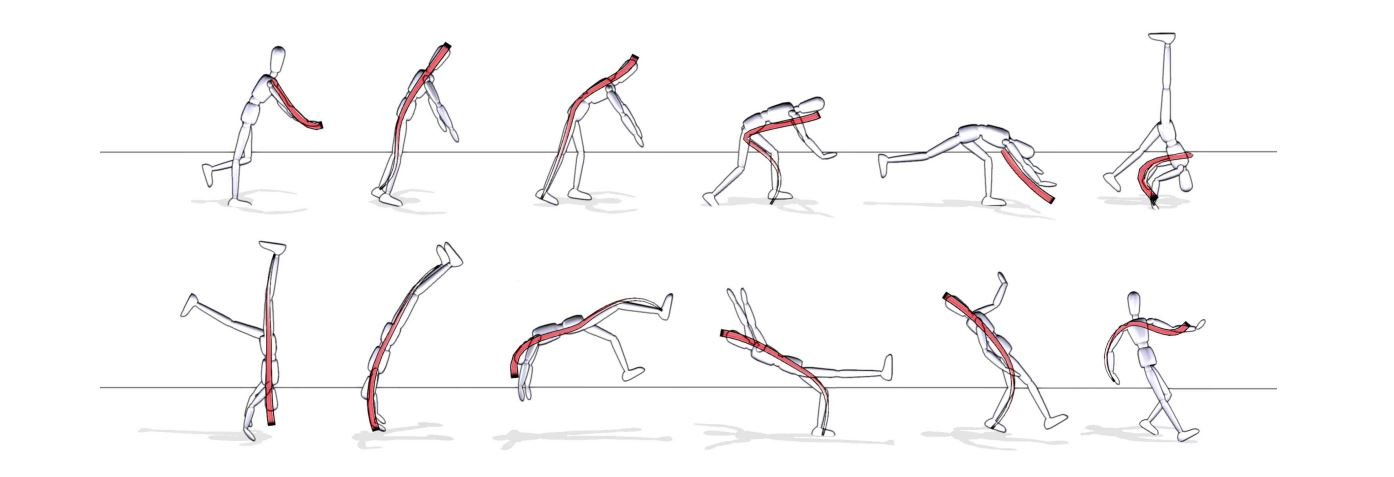
\includegraphics[scale=0.4]{img/baseline}
\caption{One character's keyframes using the line of action technique from \citep{guay2013line}.}
\end{figure}

Noticing that lines of actions can visually suggest the potential energy of a motion, Guay et. al wrote ``Adding dynamics to sketch-based character animations'' (\citep{guay2015adding})

In \citep{guay2015space}, Guay et. al continued their work on the line of action to create a technique for animation called space-time sketching, in which a user can draw a line in the path they want a model to take and it will be animated accordingly. As the character follows the path, its model bends and changes shape in a physically realistic way. Their system currently supports creating different movements with the path such as bouncing, rolling, and twisting.

Similarly, \citep{mahmudi2016artist} and \citep{stelzleni2015sketch} describe \'Ecole Polytechnique F\'ed\'erale de Lausanne's and Pixar's use of sketching to pose characters respectively. There is no mention in either paper about handling the interactions of characters. 

``SketchiMo: Sketch-based Motion Editing for Articulated Characters'' (\citep{choi2016sketchimo}) is yet another paper which takes advantage of the convenience and ease of a sketch-based interface. This time,  Choi et. al take an already saved animation and visualize the motion through time as different curves. The purpose is to allow the user to edit an existing animation, not create one. Additionally, their demo and paper focus on the animation of a single character.


\subsection{Articulated Characters}
Articulated characters are difficult to animate. Generating animation is sometimes easier than setting a character's pose over and over. The following articles explore generating animation and reusing animation.
 
FootSee: an Interactive Animation System \citep{yin2003footsee} \\

Motion Graphs \citep{kovar2002motion}\\

Style-Based Inverse Kinematics -- 2004 \citep{grochow2004style}\\
generative models for motion capture sequences used to build animations\\\\

Real-time motion retargeting to highly varied user-created morphologies\\
\citep{hecker2008real}

Using an intermediate skeleton and inverse kinematics for motion retargeting
\citep{monzani2000using}

\subsection{Physical Approach}
Displacement constraints for interactive modeling and animation of articulated structures -- 1994 \citep{gascuel1994displacement}\\

fitting geometric constraints using physics\\\\

\section{Animation of Multiple Characters}
Simulating competitive interactions using singly captured motions \citep{shum2007simulating} \\
  
A multi-resolution approach for adapting close character interaction \citep{ho2014multi} \\

Character-Object Interaction Retrieval using the Interaction Bisector Surface \citep{zhao2017character}


\section{Animation of Dancers}
\subsection{Dance Notation}
Valerie Sutton is a choreographer responsible for inventing Sutton Dance Writing, introduced in \citep{sutton1979sutton}. 

\begin{figure}[!h]
\centering
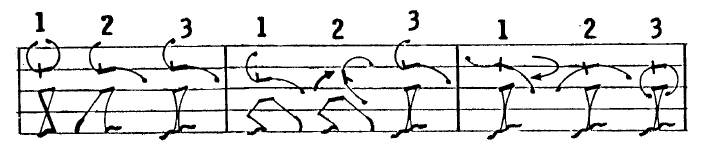
\includegraphics[scale=0.4]{img/sutton}
\caption{An example of Valerie Sutton's Dancewriting.}
\end{figure}

Benesh Movement Notation (introduced in \citep{causley1980introduction}) is analagous to Sutton notation, but for motions instead of poses.

Labanotation is another way of recording human movement.
\begin{figure}[!h]
\centering
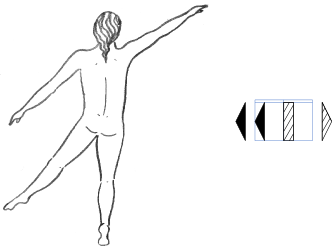
\includegraphics[scale=0.5]{img/over-labanotation}
\caption{An example of Labanotation.}
\end{figure}

\subsection{Dance in Animation}
There is a strong interest in portraying dance in animation, which can be seen in many examples of films over the years:
\begin{figure}[!h]
\centering
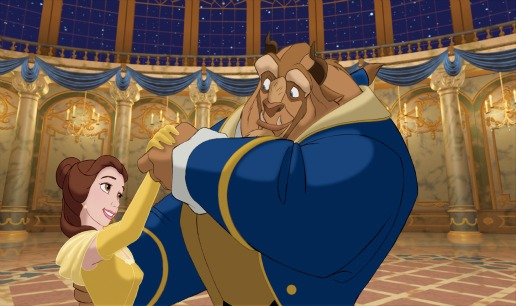
\includegraphics[scale=0.5]{img/belleetlabete}
\caption{A capture from \textit{Beauty and the Beast.}}
\end{figure}

\begin{figure}[!h]
\centering
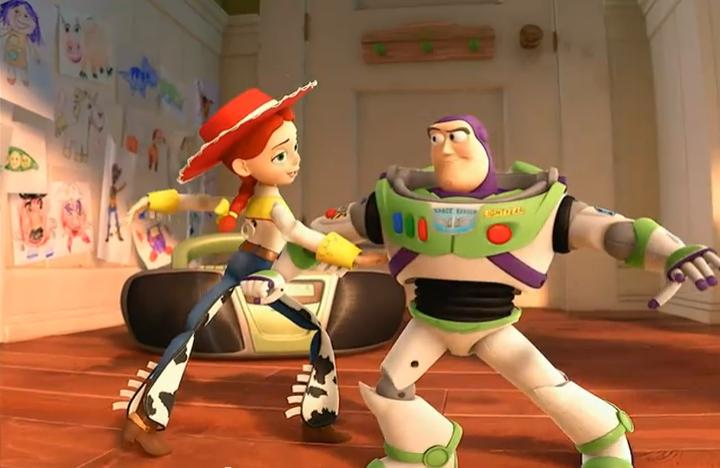
\includegraphics[scale=0.5]{img/buzz-and-jessie}
\caption{Buzz LightYear and Jessie dance.}
\end{figure}

\begin{figure}[!h]
\centering
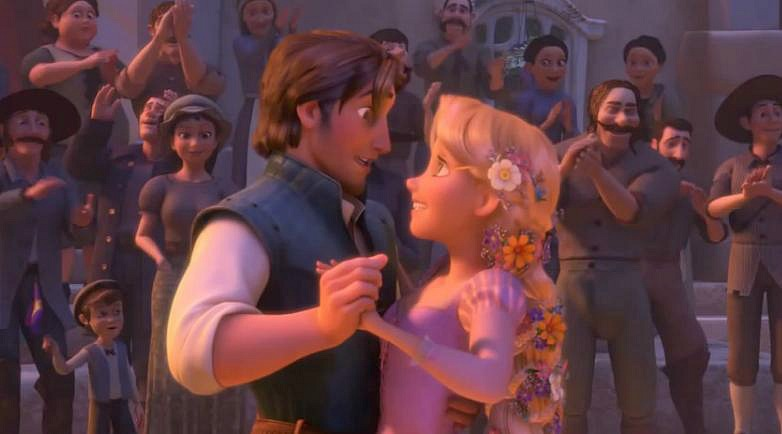
\includegraphics[scale=0.5]{img/tangled}
\caption{A scene from \textit{Tangled.}}
\end{figure}

It has progressed from live action to 2D animation to 3D animation.

So it seems almost obvious that researchers must also be interested in dance in animation. In Gleicher's 1998 paper, \citep{gleicher1998retargetting}, an application of retargetting motion from a motion capture database to 3D articulated characters of different sizes is dancing.

\begin{figure}[!h]
\centering
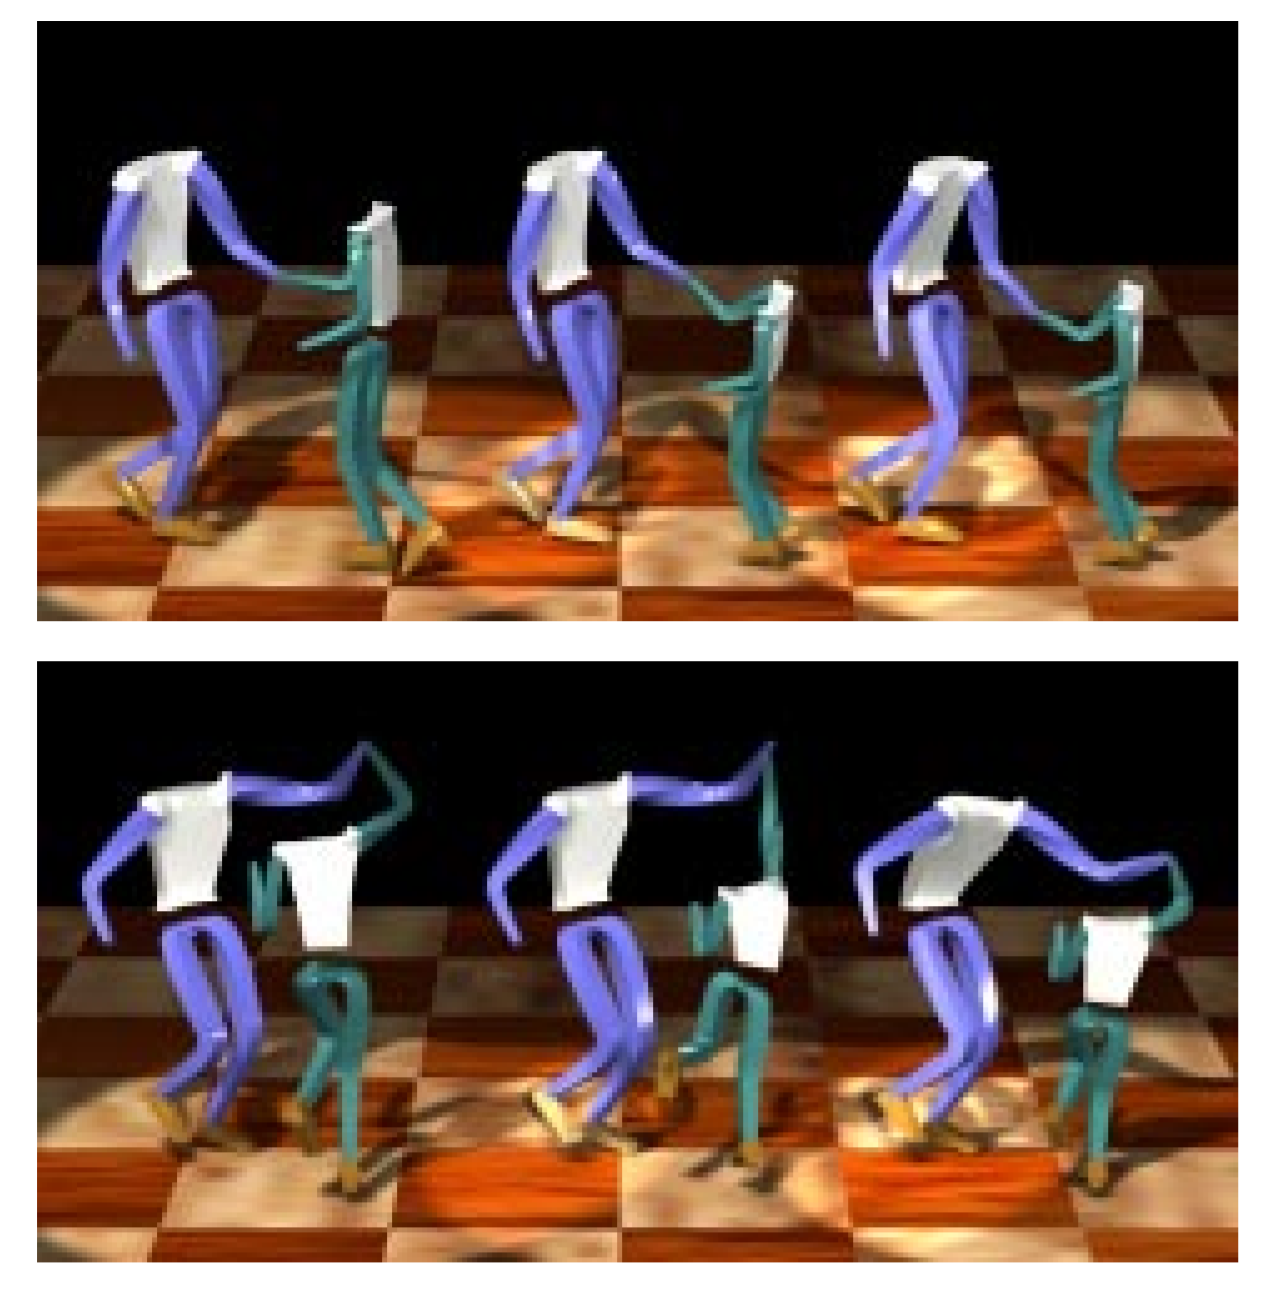
\includegraphics[scale=0.5]{img/retarget}
\caption{Motion retargetting applied to dance from \citep{gleicher1998retargetting}.}
\end{figure}

Based on the 2005 paper \citep{calvert2005applications}, Matthews et. al experimented with generating dance motion in the paper \citep{matthews2011procedural}. \citep{shiratori2006dancing} and \citep{shiratori2006synthesizing} synthesize music and an animation generated from a motion graph built from motion capture data.
